\section{问题三的模型的建立和求解}
\subsection{问题三的描述与分析}

\subsection{预备工作}


为适配附件三的多微基站、同频复用且存在小区间干扰的场景,定义如下集合与索引:

\begin{itemize}
  \item 基站集合:$\mathcal{N}=\{1,2,3\}$(分别对应 BS1、BS2、BS3)。
  \item 切片集合:$\mathcal{S}=\{U,e,m\}$,分别对应 URLLC、eMBB、mMTC。
  \item 用户集合:$\mathcal{K}=\mathcal{K}_U\cup\mathcal{K}_e\cup\mathcal{K}_m$,其中 $\mathcal{K}_U=\{\mathrm{U1},\mathrm{U2}\}$,$\mathcal{K}_e=\{\mathrm{e1},\dots,\mathrm{e12}\}$,$\mathcal{K}_m=\{\mathrm{m1},\dots,\mathrm{m30}\}$。
  \item 决策时刻集合:$\mathcal{T}=\{0,100,\dots,900\}$(单位 ms),每个决策窗口长度为 $100$ ms;窗口内以 $1$ ms 步长进行链路与队列仿真,记窗口内细粒度时刻集合为 $\mathcal{F}(t)=\{t,t+1,\dots,t+99\}$。
\end{itemize}

其余关键系统参数与问题一、二保持一致。

\subsection{模型建立}
问题三的基本模型与问题二一致,但是需要考虑多个微基站之间的信号干扰,故需要对信道与干扰模型进行重新建模,其余复用模型不再重复。

\subsubsection{信道与干扰模型}

附件三提供了每 $1$ ms 的大规模损耗 $\phi_{n,k}(\tau)$(dB)与小规模瑞利衰落 $h_{n,k}(\tau)$。设窗口 $t\in\mathcal{T}$ 内细粒度时刻为 $\tau\in\mathcal{F}(t)$,若用户 $k\in\mathcal{K}_s$ 在窗口 $t$ 由基站 $n$ 服务且被分配切片 $s$ 的 RB,则其接收功率(mW)为
\begin{equation}
 p_{\mathrm{rx},n\to k}(\tau)=10^{\frac{p_{n,s}(t)-\phi_{n,k}(\tau)}{10}}\cdot |h_{n,k}(\tau)|^2.
\end{equation}

噪声功率与占用 RB 数 $i$ 成正比,换算为线性功率(mW):
\begin{equation}
 N_0(i)=10^{\frac{-174+10\log_{10}(i\cdot b)+NF-30}{10}}.
\end{equation}

微基站同频复用引入同信道干扰。为保持“同一 RB 索引才互扰”的规则,我们令每站在窗口 $t$ 内将其 $50$ 个 RB 在频域上按切片连续划分且次序固定(例如 U-e-m),每个切片获得一段连续 RB 区间,跨站的相同 RB 索引构成同信道。于是用户 $k$ 的瞬时信干噪比为
\begin{equation}
 \gamma_k(\tau)=\frac{p_{\mathrm{rx},n\to k}(\tau)}{\sum\limits_{u\in\mathcal{N},\ u\neq n} I_{u\to k}(\tau)+N_0(i_s)},\quad s\in\mathcal{S},
\end{equation}
其中 $I_{u\to k}(\tau)$ 表示来自他站 $u$、在与 $k$ 所占 RB 索引重叠的切片 RB 上的干扰功率,按与上式相同的接收功率表达(由 $p_{u,s'}(t),\phi_{u,k}(\tau),h_{u,k}(\tau)$ 决定)。基于香农公式,窗口内瞬时速率为
\begin{equation}
 r_k(\tau)=i_s\cdot b\cdot \log_2\big(1+\gamma_k(\tau)\big)\quad(\mathrm{bps}).
\end{equation}
\subsubsection{任务到达与队列演化}

任务队列的动态演化过程与问题二完全一致,队列状态 $Q_k(t)$ 仍以每个用户为中心进行追踪,其演化遵循公式 \eqref{eq:queue_evolution}。

关键区别在于,服务量 $S_k(t)$ 的计算变得更为复杂,因为它取决于用户 $k$ 在当前窗口 $t$ 接入了哪个基站 $n$,以及所有基站的功率决策 $\{p_{n,s}(t)\}$。这将在后续的服务质量评估函数中具体体现。


\subsubsection{决策变量与优化模型}

决策变量:
\begin{itemize}
  \item RB 切片分配:$x_{n,s}(t)\in\mathbb{Z}_{\ge 0}$
  \item 发射功率:$p_{n,s}(t)\in[10,30]\,\mathrm{(dBm)}$
  \item 接入关联:$a_{n,k}(t)\in\{0,1\}$,当 $a_{n,k}(t)=1$ 则 $k$ 在窗口 $t$ 仅由站 $n$ 调度
\end{itemize}

综合上述要素,第三问的动态联合优化模型可表述为(跨 10 个窗口聚合):
\begin{equation}
\begin{aligned}
\max_{\{x,p,a\}}\quad & Q_{\text{total}}=\sum_{t\in\mathcal{T}}\Bigg[\sum_{k\in\mathcal{K}_U}\sum_{\tau\in\mathcal{A}_k(t)} y^{U}_{k,\tau}+\sum_{k\in\mathcal{K}_e}\sum_{\tau\in\mathcal{A}_k(t)} y^{e}_{k,\tau}+\sum_{k\in\mathcal{K}_m}\sum_{\tau\in\mathcal{A}_k(t)} y^{m}_{k,\tau}\Bigg] \\
\text{s.t.}\quad & 
\left\{
\begin{aligned}
&\sum_{s\in\mathcal{S}} x_{n,s}(t)=50 \\
&x_{n,U}(t)\bmod 10=0 ,x_{n,e}(t)\bmod 5=0 ,x_{n,m}(t)\bmod 2=0 \\
&x_{n,s}(t)\in\mathbb{Z}_{\ge 0} \\
&10\le p_{n,s}(t)\le 30\\
&Q_k(t+100)=\max\Big\{0,\ Q_k(t)+\sum_{\tau\in\mathcal{F}(t)} D_k(\tau)-S_k(t)\Big\} \\
&r_k(\tau),\ \gamma_k(\tau)\ \text{由}\ (x,p,a)\ \text{与}\ (\phi,h)\ \text{及调度生成} \\
&\sum_{n\in\mathcal{N}} a_{n,k}(t)\le 1 \\
&\forall n\in\mathcal{N},\ t\in\mathcal{T},\ \forall n,k,s,t
\end{aligned}
\right.
\end{aligned}
\end{equation}
其中 $\mathcal{A}_k(t)\subseteq\mathcal{F}(t)$ 为窗口 $t$ 内属于用户 $k$ 且在 SLA 内完成的任务到达时刻集合;$r_k(\tau)$ 与 $S_k(t)$ 均受干扰耦合与调度影响,是 $(x,p,a)$ 的非线性函数。\\
该模型体现了“多站同频干扰 + 切片化 RB 分配 + 切片级功率控制 + 任务队列”的耦合特性,属于带整数约束与非凸干扰项的时变 MINLP 问题。

\subsection{模型求解}
针对第三问的模型,我们分析得到:
1) 决策维度急剧扩张,包含了 9 个连续的功率变量 $\{p_{n,s}\}$ 与 48 个离散的用户接入基站变量 $\{a_{n,k}\}$,构成了庞大的混合搜索空间。
2) 小区间干扰项使目标函数呈现强非凸、非线性特性,枚举或传统凸优化方法难以求解,计算量将呈指数级爆炸。
故,前两问的“切片 RB 枚举 + 预测–控制 (MPC)”框架无法直接扩展到第三问。

为兼顾求解质量与计算效率,本文不再使用枚举仿真的方法,而是引入启发式算法,快速找到近似最优解。本问采用“\textbf{滚动时窗预测控制(MPC)}+\textbf{混合编码遗传算法(GA)}”的两层求解方法。

\subsubsection{外层:滚动时窗预测控制 (MPC)}
我们将 1000 ms 的总时长离散为 10 个长度为 $T_w=100$ ms 的独立决策窗口。在每个窗口 $t$ 的开始,我们求解一个静态优化问题,以确定该窗口内恒定不变的资源分配策略(包括用户接入、RB切片、功率等级)。这种滚动优化的方式使得模型可以应对时变的信道和业务\upcite{SSJDEBA60604345B90069821C30F1E772659}。


\subsubsection{内层:混合编码遗传算法 (GA)}
针对每个窗口内的静态资源分配问题,我们设计了遗传算法进行启发式搜索。GA 能够有效处理高维、非凸、含混合变量的复杂优化问题\upcite{JSJA2024S1161}。
\begin{itemize}
    \item \textbf{个体编码方案}:每个个体(染色体)代表一个完整的资源分配策略,采用混合编码,由三部分组成:
    \begin{enumerate}
        \item \textbf{用户接入决策}:长度为 48 的整数向量,每个基因位代表一个用户,其值(0, 1, 2)表示该用户接入的基站(BS1, BS2, BS3)。
        \item \textbf{RB 切片分配}:长度为 6 的整数向量,每两位表示一个基站为 URLLC 和 eMBB 切片分配的 RB 数量。mMTC 切片的比例则由剩余资源确定,并根据切片粒度约束进行解码。
        \item \textbf{切片功率控制}:长度为 9 的浮点数向量,每个基因位表示一个基站上特定切片(U/E/M)的发射功率(dBm),范围在 $[10, 30]$。
    \end{enumerate}
    \item \textbf{适应度函数}:个体的适应度由一个精细的仿真器评估。该仿真器将个体解码后的策略作为输入,以 1 ms 为步长模拟整个 100 ms 窗口的动态过程。仿真完整地计算了用户速率(包含所有基站的同频干扰)、任务队列的演化以及最终产生的 QoS 总分。该 QoS 总分即为个体的适应度。
    \item \textbf{遗传算子与参数}:
    GA 采用精英保留策略,并使用锦标赛选择、算术交叉(针对连续变量)/单点交叉(针对离散变量)和高斯/随机扰动变异(针对不同类型变量)来产生新一代种群。关键参数设置如下:种群大小为 40,最大进化代数为 200,精英个体保留 5 个,交叉概率 0.8,变异概率 0.3。
\end{itemize}
\subsubsection{求解流程}
本算法采用“滚动时窗预测控制”框架,将1000ms划分为10个独立的100ms优化窗口。每个窗口内,利用遗传算法(GA)进行静态资源分配优化,简要流程如图~\ref{fig:flow_q3}所示。

\begin{figure}[H]
  \centering
  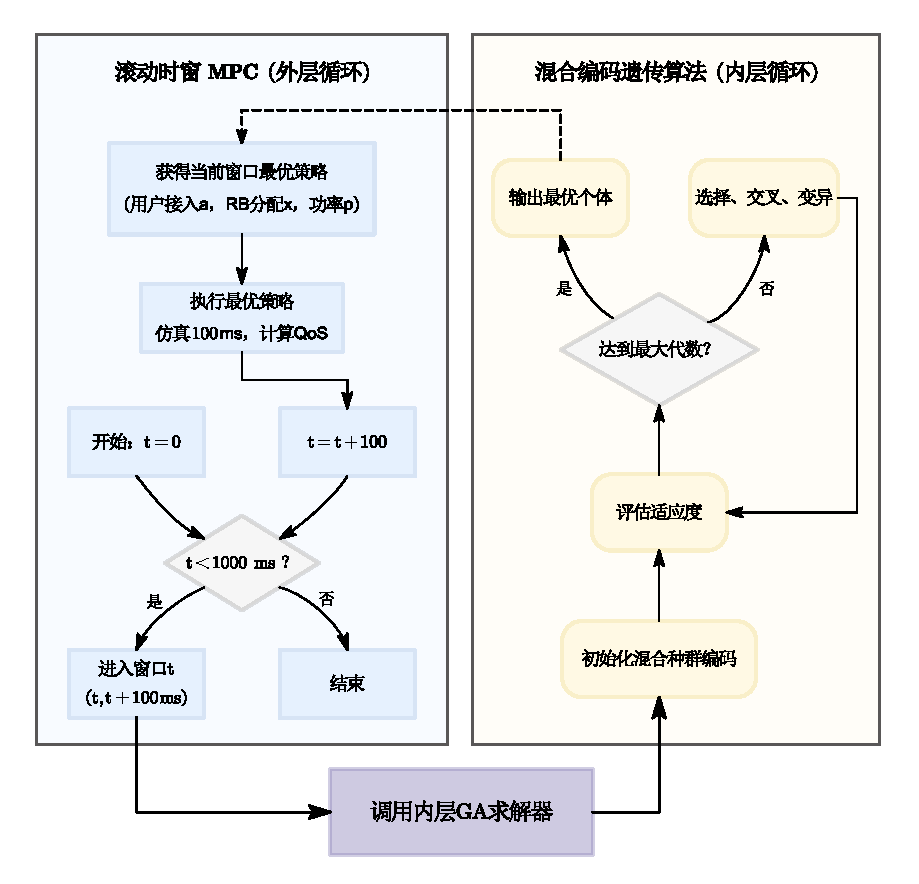
\includegraphics[width=0.9\textwidth]{figures/第三问算法.pdf}
  \caption{问题三“滚动 MPC + GA”求解流程图}
  \label{fig:flow_q3}
\end{figure}

\subsection{结果分析}
我们采用上一节提出的“滚动MPC+GA”方法对问题三进行了求解,得到了10个决策窗口内每个基站的资源块(RB)分配、切片功率以及用户接入策略。详细的数值结果记录在代码附录的 \texttt{q3\_user\_bs\_mapping.csv} 和 \texttt{q3\_window\_results.csv} 文件中。本节将对这些结果进行分析。

\subsubsection{总体性能与动态适应性}
在1000ms的仿真周期内,我们所提出的算法实现了 \textbf{871.34} 的总服务质量(QoS)得分。每个窗口的详细QoS得分、资源和功率分配决策汇总于表~\ref{tab:q3_results}。

\begin{table}[H]
  \centering
  \caption{问题三各窗口资源分配决策与QoS结果}
  \label{tab:q3_results}
  \resizebox{\textwidth}{!}{%
  \begin{tabular}{c|ccc|ccc|ccc|ccc|c}
    \toprule
    \textbf{Win} & \multicolumn{3}{c|}{\textbf{BS1 (RB/P(dBm))}} & \multicolumn{3}{c|}{\textbf{BS2 (RB/P(dBm))}} & \multicolumn{3}{c|}{\textbf{BS3 (RB/P(dBm))}} & \multicolumn{3}{c|}{\textbf{QoS}} & \textbf{Obj.} \\
    \cmidrule(lr){2-4} \cmidrule(lr){5-7} \cmidrule(lr){8-10} \cmidrule(lr){11-13}
     & \textbf{U} & \textbf{E} & \textbf{M} & \textbf{U} & \textbf{E} & \textbf{M} & \textbf{U} & \textbf{E} & \textbf{M} & \textbf{U} & \textbf{E} & \textbf{M} & \\
    \midrule
    0 & 0/24.4 & 40/22.8 & 10/24.8 & 20/21.6 & 0/22.9 & 30/23.4 & 20/21.6 & 0/22.9 & 30/21.7 & 38.16 & 8.40 & 30.00 & 76.56 \\
    1 & 10/21.1 & 0/21.0 & 40/25.6 & 10/20.2 & 20/24.2 & 20/20.9 & 20/21.7 & 20/24.3 & 10/23.2 & 51.03 & 6.81 & 30.00 & 87.84 \\
    2 & 10/21.9 & 0/20.1 & 40/25.1 & 0/18.9 & 40/25.4 & 10/22.7 & 20/20.5 & 0/24.8 & 30/21.0 & 38.35 & 9.87 & 30.00 & 78.22 \\
    3 & 30/19.9 & 0/22.5 & 20/18.0 & 20/20.4 & 0/20.3 & 30/22.4 & 0/19.4 & 30/23.7 & 20/20.2 & 49.26 & 7.79 & 30.00 & 87.05 \\
    4 & 10/23.2 & 20/26.2 & 20/24.0 & 30/21.6 & 0/20.7 & 20/21.6 & 10/20.5 & 0/21.8 & 40/22.2 & 46.43 & 5.90 & 30.00 & 82.33 \\
    5 & 0/19.2 & 30/24.1 & 20/21.4 & 20/21.3 & 0/21.3 & 30/20.2 & 30/22.4 & 0/21.3 & 20/22.8 & 52.02 & 7.28 & 30.00 & 89.30 \\
    6 & 10/21.9 & 0/21.3 & 40/20.6 & 10/22.5 & 0/21.5 & 40/22.7 & 20/21.3 & 20/25.5 & 10/21.0 & 52.08 & 6.25 & 30.00 & 88.33 \\
    7 & 10/21.6 & 0/22.9 & 40/22.0 & 10/19.2 & 20/26.2 & 20/17.5 & 20/24.7 & 0/21.5 & 30/20.6 & 48.68 & 6.40 & 30.00 & 85.08 \\
    8 & 20/22.5 & 0/18.6 & 30/22.9 & 20/18.7 & 0/17.9 & 30/23.3 & 10/22.3 & 20/29.8 & 20/23.0 & 51.45 & 7.59 & 30.00 & 89.04 \\
    9 & 0/21.4 & 30/27.3 & 20/22.7 & 30/24.5 & 0/22.0 & 20/20.7 & 10/21.6 & 0/23.2 & 40/21.1 & 56.80 & 7.88 & 30.00 & 94.69 \\
    \bottomrule
  \end{tabular}%
  }
\end{table}
结果显示,算法能够根据每个窗口变化的信道条件和任务到达情况,动态调整资源分配策略。
\subsubsection{用户接入策略}
程序在每次决策时,会根据当前信道条件和任务到达情况,选择一个基站为用户提供服务。
图~\ref{fig:q3_first_window_vis} 展示了第一次决策窗口内用户接入与资源分配的可视化结果。
\begin{figure}[H]
    \centering
    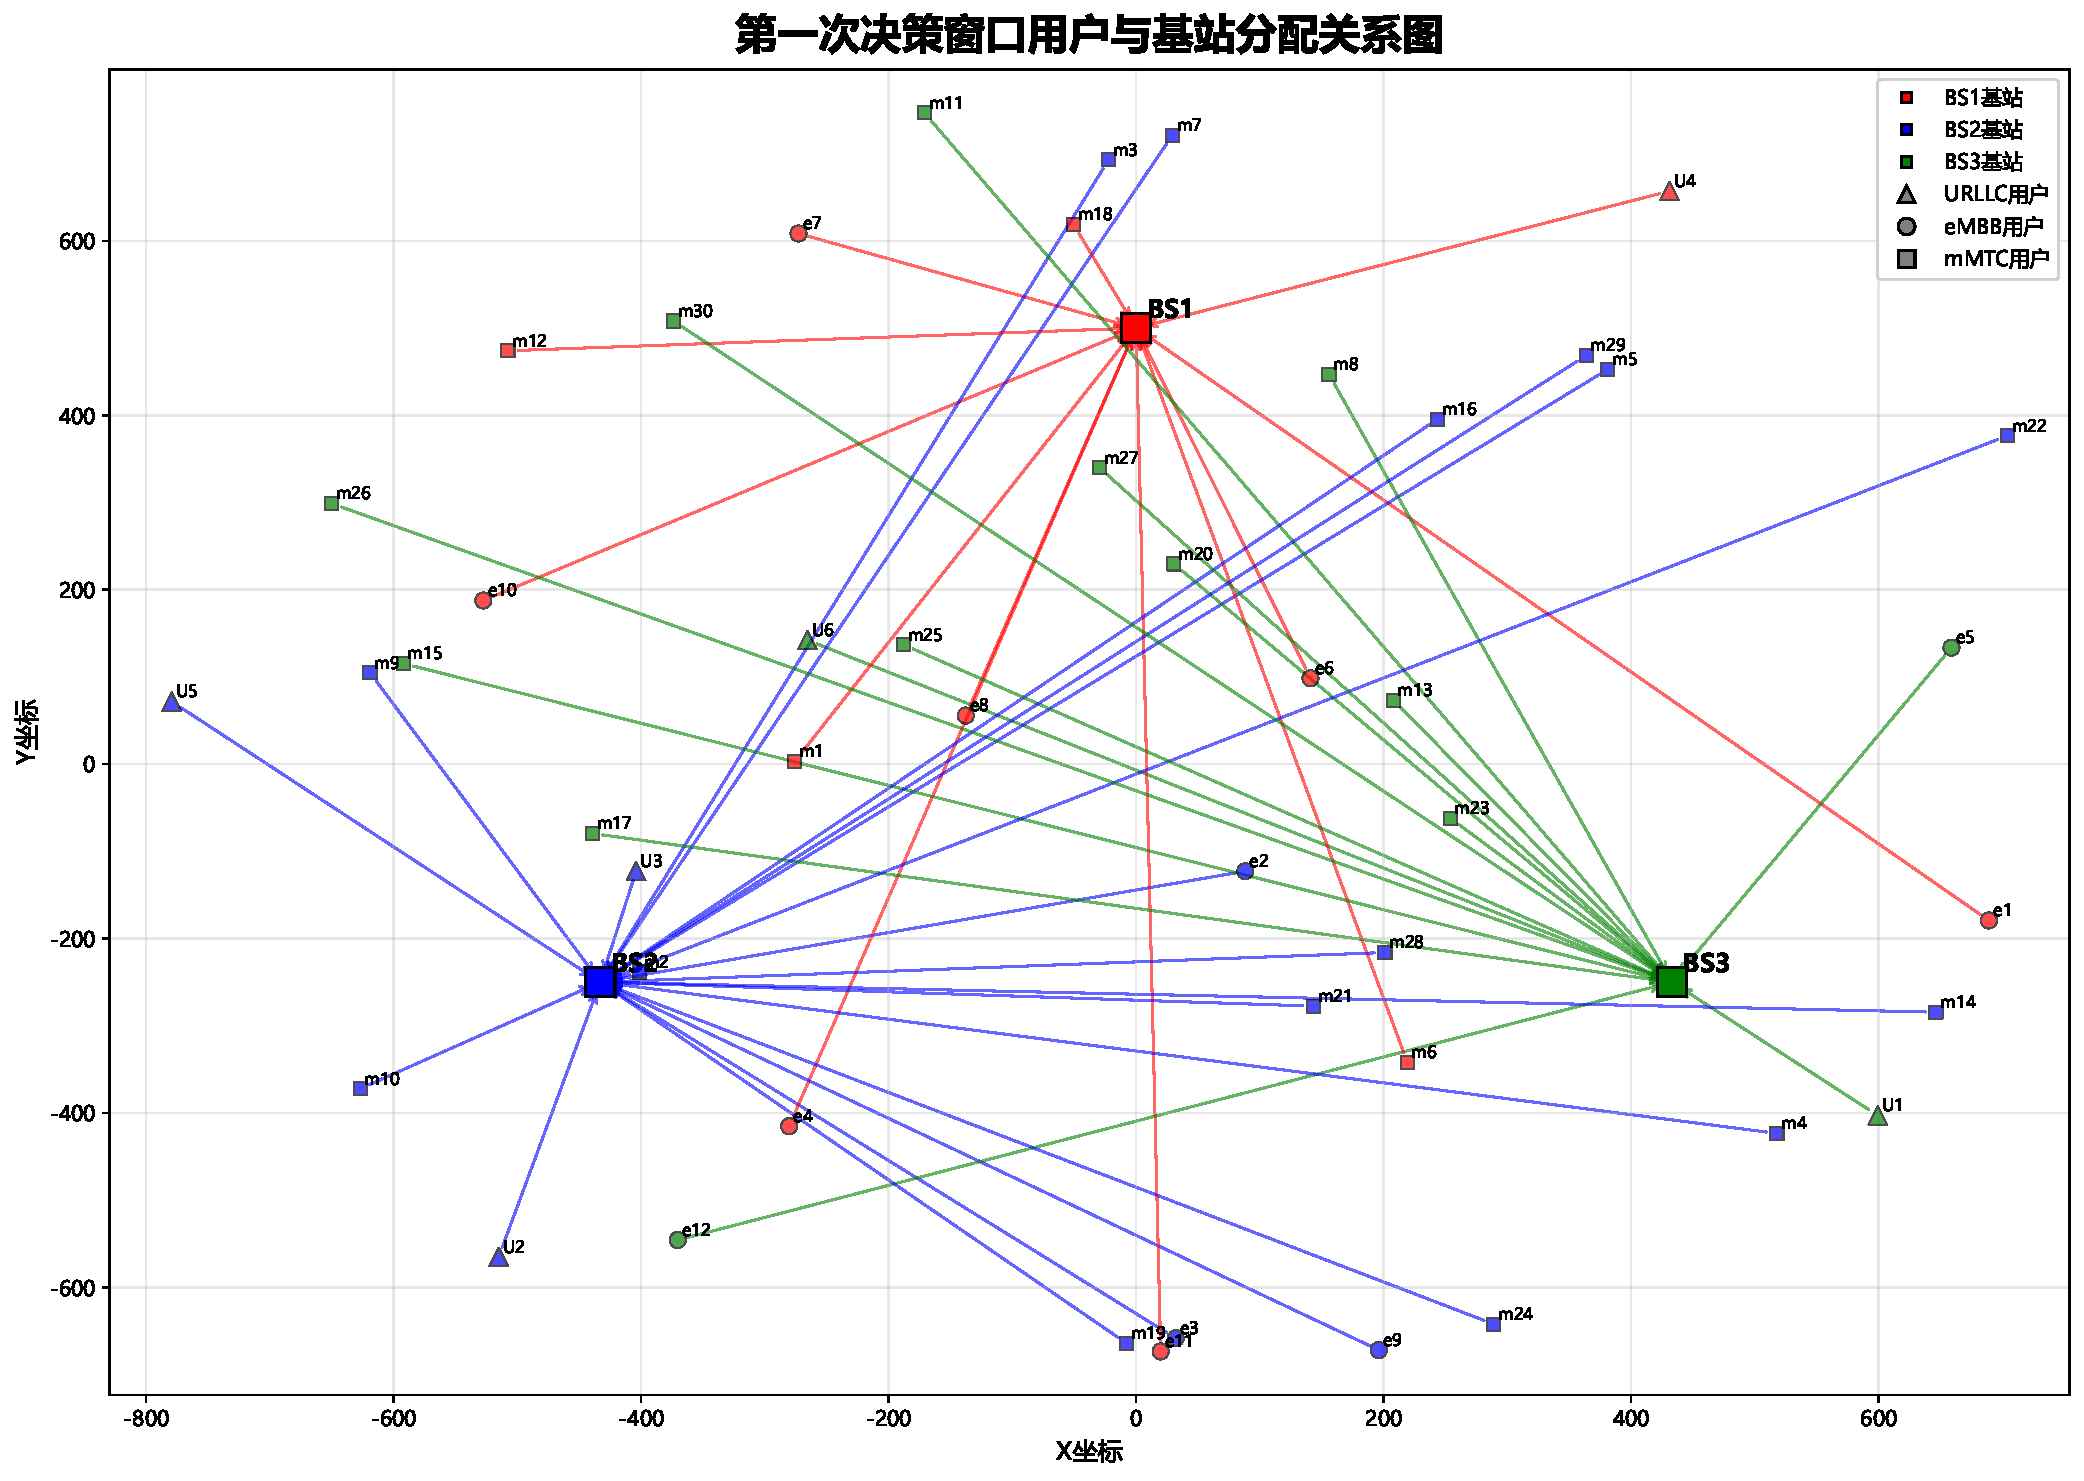
\includegraphics[width=0.85\textwidth]{figures/第一次决策可视化.pdf}
    \caption{第一次决策窗口用户接入可视化}
    \label{fig:q3_first_window_vis}
\end{figure}

\subsubsection{切片资源分配与干扰管理策略}
遗传算法在每个窗口内搜索“用户接入+RB分配+功率控制”的联合最优解,其分配策略体现了对不同切片QoS需求的深刻理解和对干扰的精细化控制。
\begin{itemize}
    \item \textbf{URLLC (U-slice)}:作为最高优先级的业务,其QoS得分(sum\_U)在各个窗口都获得了较高的满足度。算法倾向于为其分配较高的发射功率(如窗口8中BS3的29.8dBm),以克服路径损耗和干扰,确保其超低时延和高可靠性要求。当URLLC任务负载较重时(如窗口9),算法会聚合多个基站的资源(BS2分配30个RB,BS3分配10个RB)来共同满足需求。
    \item \textbf{eMBB (E-slice)}:该切片追求高吞吐量,对SINR敏感。算法的决策体现了机会主义调度思想:当某个基站与某些eMBB用户之间的信道条件极好,且来自邻近基站的干扰较小时,会大胆地为其分配大量RB和较高的功率(如窗口9中BS1为eMBB分配30个RB,功率高达27.3dBm)。反之,若信道或干扰环境恶劣,则会减少资源分配,避免资源浪费。
    \item \textbf{mMTC (M-slice)}:该切片服务质量目标是“尽力而为”地满足所有用户的基本连接需求。从结果看,几乎所有窗口的mMTC QoS得分都达到了其上限30分,表明算法总能找到足够的“边角料”资源来满足海量但低速率的连接请求,实现了对网络资源的充分利用。
\end{itemize}




